\subsection*{Энтропийное кодирование}~\
	
Как говорилось ранее, энтропия показывает наименьшее среднее число бит, необходимое для кодирования некоторой информации. Данное свойство используется, как ни странно, при кодировании информации.
	
Например, код Шеннона-Фано. С целью минимизации энтропии и, соответственно, оптимизации кода элементы с большой вероятностью появления кодируются меньшим числом символом. Таким образом, производится сжатие объема информации, что позволяет передавать большее количество информации, затрачивая меньший объем памяти.
	
\subsection*{Построение решающих деревьев}~\
	
Решающие деревья --- метод, использующийся в машинном обучении и работающий по принципу принятия решений человеком. Каждое ветвление представляет собой разделение выборки на две части по порогу некоторого признака. Например, признак --- длина, пороговое значение ---  38. Все объекты, длина которых превышает 38, отделяются от объектов с длиной меньше 38 и дальнейший анализ проходят отдельно.
	\begin{center}
	\tikzstyle{level 1}=[level distance=1cm, sibling distance=5cm]
	\tikzstyle{level 2}=[level distance=1cm, sibling distance=1cm]
	\tikz
	\node {Длина < 38 попугаев}
	child { node {Да}
		child { node {Обыкновенный удав}}}
	child { node {Нет}
		child { node {Анаконда}}};
	\end{center}
	В данном методе расчет энтропии помогает определить оптимальный порог для каждого узла решения. А именно, подбирается такое разделение выборки, при котором сумма энтропий получившихся выборок минимальна среди возможных вариантов разбиений.
	
	Например, у нас есть выборка объектов с одним признаком, длина: 22 попугая (обыкновенный удав), 46 попугаев (анаконда), 40 попугаев (анаконда), 31 попугай (обыкновенный удав). Мы выбираем порог: 38 или 44 попугаев?
	Попробуем разделить выборку по 38 попугаям:
	\begin{center}
	\tikzstyle{level 1}=[level distance=1cm, sibling distance=7cm]
	\tikzstyle{level 2}=[level distance=1cm, sibling distance=1cm]
	\tikz
	\node {Длина < 38 попугаев}
	child { node {Да}
		child { node {Обыкновенный удав, обыкновенный удав}}}
	child { node {Нет}
		child { node {Анаконда, анаконда}}};
	\end{center}

	При расчете энтропии $0 \cdot \log_2 0$ считается равным 0, несмотря на $\log_2 0$. За вероятность принимается вероятность встретить данный класс в новой выборке.
	
	Энтропия левой части: $-(1 \cdot \log_2 1 + 0 \cdot \log_2 0) = 0$. Энтропия правой части: $-(1 \cdot \log_2 1 + 0 \cdot \log_2 0) = 0$. Суммарная энтропия получилась: $0$.
	
	Попробуем разделить выборку по 44 попугаям:
	\begin{center}
	\tikzstyle{level 1}=[level distance=1cm, sibling distance=7cm]
	\tikzstyle{level 2}=[level distance=1cm, sibling distance=1cm]
	\tikz
	\node {Длина < 44 попугаев}
	child { node {Да}
		child { node {Обыкновенный удав, анаконда, обыкновенный удав}}}
	child { node {Нет}
		child { node {Анаконда}}};
	\end{center}

	Энтропия левой части: $-(\frac{1}{3} \cdot \log_2 \frac{1}{3} + \frac{2}{3} \cdot \log_2 \frac{2}{3}) \approx 0.92 $.
	Энтропия правой части: $-(1 \cdot \log_2 1 + 0 \cdot \log_2 0) = 0$. Суммарная энтропия получилась: $0.92$.
	
	В первом случае мы идеально разделили выборку при энтропии, равной нулю. Во втором случае нам удалось отделить одну анаконду, но не удалось отделить классы. Так и энтропия в первом случае оказалась меньше, чем во втором. Причем ее равенство нулю необязательно --- любое значение меньше 0.92 показало бы, что первый случай более оптимален. Здесь же, в виду неотрицательности энтропии, однозначно можно сказать, что критерий <<длина < 38 попугаев>> дает оптимальный результат.
	
	Энтропия позволяет получать после разбиения выборки, наименее разнообразные по содержанию классов (менее хаотичные). Соответственно, признак и пороговое значение подбираются наиболее оптимально --- алгоритм успешно отделяет объекты, принадлежащие к одному классу.
	
\subsection*{Применение в алгоритмах t-SNE и UMAP}~\
	\\
	
	В анализе данных часто возникает необходимость в снижении размерности, и в таких случаях на помощь приходят знания об энтропии. Речь, конечно, идет не об энтропии как таковой, а об алгоритмах, которые базируются на теории.
	
	При создании пространства меньшей размерности, t-SNE и UMAP используют кросс-энтропию как показатель эффективности перенесения свойств объектов. Чем меньше кросс-энтропия, тем ближе к истинному оказалось подобранное распределение.
	
	Приведем пример работы алгоритма UMAP. Мы возьмем набор данных об одежде, который включает в себя 70000 черно-белых изображений различной одежды по 10 классам: футболки, брюки, свитеры, платья, кроссовки и т.д. Каждая картинка имеет размер 28x28 пикселей или 784 пикселя.
	
	Изначально каждый пиксель является признаком объекта (фотографии) и принимает некоторое значение (цвет). Если бы каждая картинка состояла из двух пикселей, мы бы смогли построить график, где по оси абсцисс отложен цвет одного пикселя, по оси ординат цвет второго пикселя, и изобразить точками все объекты.
	
	У нас каждая картинка состоит из 784 пикселей --- 784-мерное пространство, поэтому изобразить его проблематично. Но если мы преобразуем выборку таким образом, что останется всего два признака, то мы сможем визуализировать ее. Получившиеся признаки будут уже не пикселями, а абстрактными признаками, которые алгоритм получает из исходных --- переводит 784 признака в 2 с помощью функции, подобранной в результате работы.
	
	Реализуем описанный алгоритм\footnote{Реализация позаимствована из \url{https://github.com/lmcinnes/umap/blob/master/doc/supervised.rst}}.
	
	Внимание! Библиотека UMAP требует предварительной установки\footnote{Почитать про установку: \url{https://umap-learn.readthedocs.io/en/latest/}}.
	
	Импортируем нужные библиотеки:
	\begin{minted}{Python}
import numpy as np # работа с матрицами
from mnist import MNIST # наборы данных
import matplotlib.pyplot as plt # построение графиков
%matplotlib inline
import umap # алгоритм UMAP
	\end{minted}
	
	Загружаем набор данных с фотографиями одежды.
	\begin{minted}{Python}
mndata = MNIST('fashionmnist')
train, train_labels = mndata.load_training() 
test, test_labels = mndata.load_testing()
data = np.array(np.vstack([train, test]), dtype=np.float64) / 255.0
target = np.hstack([train_labels, test_labels])
	\end{minted}

	Cоздаем список из наименований одежды.
\begin{minted}{Python}
classes = ['T-shirt/top', 'Trouser', 'Pullover', 'Dress', 'Coat', 'Sandal', 
'Shirt', 'Sneaker', 'Bag', 'Ankle boot']
\end{minted}

Запускаем UMAP.
\begin{minted}{Python}
embedding = umap.UMAP().fit_transform(data)
\end{minted}

Визуализируя результат, получаем:

\begin{figure}[bh]
	\noindent\centering{
		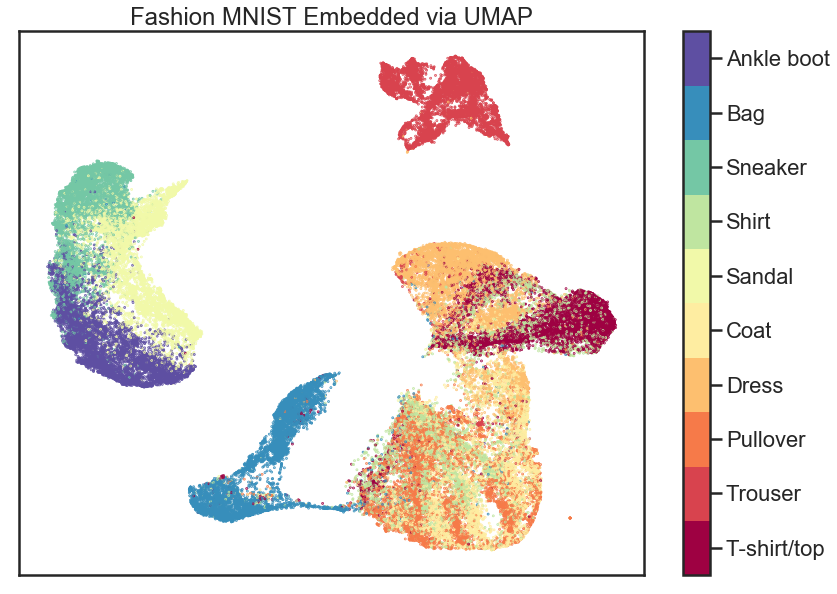
\includegraphics[height=70mm, width=110mm]{umap.png}
	}
	\caption{Алгоритм UMAP}
	\label{figCurves}
\end{figure} 

Получить два новых признака из исходных можно очень многими способами. Но они должны описывать выборку как можно лучше, чтобы при визуализации мы видели не случайно нарисованное изображение, а отображение начального пространства.

Именно тут алгоритм применяет кросс-энтропию. Однако не совсем обычную, а кросс-энтропию нечетких множеств\footnote{Нечеткое множество --- множество, элементы которого принадлежат ему с некоторой вероятностью.}, которая показывает, насколько одно множество отличается от другого. UMAP --- алгоритм, выполняющий построение ориентированного взвешенного графа, чтобы перевести его в низкоразмерное пространство. Поэтому в нашем случае нечеткие множества состоят из ребер, соединяющих объекты --- ребро между двумя объектами может либо существовать с вероятностью $w$, либо не существовать с вероятностью $1-w$, где $w$ --- вес ребра в исходном пространстве.

Энтропия нечетких множеств отличается от обычной энтропии для дискретных случайных величин тем, что вместо вероятностей записывается функция принадлежности элемента к множеству. Кросс-энтропия содержит в себе отношение двух функций принадлежности множеств, которые мы сравниваем. Формула для UMAP сравнивает одно и то же множество, но с разными функциями принадлежности, соответствующими высокоразмерному ($w$) и низкоразмерному пространствам ($t$):

\[C\left[(M, w(m)), (M, t(m))\right] = \sum_{m \in M} \left(w(m) \log \left[\cfrac{w(m)}{t(m)}\right] + (1 - w(m)) \log \left[\cfrac{1 - w(m)}{1 - t(m)}\right]\right)\]

Например, пусть у нас есть выборка из 5 объектов, и мы знаем веса ребер между ними в исходном пространстве:
\begin{center}
	\begin{tabular}{|c||c|c|c|c|c|}
		\hline
		& D & Y & L & M & O\\
		\hline
		\hline
		D & - & - & 0.42 & 0.17 & 0.99\\
		\hline
		Y & - & - & 0.38 & 0.99 & 0.21\\
		\hline
		L & 0.1 & - & - & 0.74 & 0.74 \\
		\hline
		M & - & 0.74 & 0.74 & - & 0.1 \\
		\hline 
		O & 0.74 & - & 0.74 & 0.1 & -\\
		\hline 
	\end{tabular}
\end{center}

UMAP выполняет автоматическую минимизацию кросс-энтропии. Поскольку вручную данное действие выполнить сложно, то мы можем попробовать подобрать $t(m)$, выбирая из нескольких множеств:

\begin{center}
	\begin{multicols}{2}
		\begin{tabular}{|c||c|c|c|c|c|}
			\hline
			$t_1$ & D & Y & L & M & O \\
			\hline
			\hline
			D & - & - & 0.21 & 0.43 & 0.94 \\
			\hline
			Y & - & - & 0.34 & 0.73 & 0.51 \\
			\hline
			L & 0.21 & - & - & 0.7 & 0.67 \\
			\hline
			M & - & 0.74 & 0.74 & - & 0.1 \\
			\hline 
			O & 0.15 & - & 0.44 & 0.99 & - \\
			\hline 
		\end{tabular}\\
		\begin{tabular}{|c||c|c|c|c|c|}
			\hline
			$t_2$ & D & Y & L & M & O\\
			\hline
			\hline
			D & - & - & 0.09 & 0.85 & 0.64\\
			\hline
			Y & - & - & 0.4 & 0.22 & 0.96\\
			\hline
			L & 0.22 & - & - & 0.7 & 0.66\\
			\hline
			M & - & 0.32 & 0.36 & - & 0.9 \\
			\hline 
			O & 0.25 & - & 0.34 & 0.99 & -\\
			\hline 
		\end{tabular}
	\end{multicols}
\end{center}

Кросс-энтропия для $t_1(m)$:
\[C[(M, w(m)), (M, t_1(m))] = 0.42\log \frac{0.42}{0.21} + (1-0.42)\log \frac{1-0.42}{1-0.21} + \cdots \approx 5.7\]

Кросс-энтропия для $t_2(m)$:
\[C[(M, w(m)), (M, t_2(m))] = 0.42\log \frac{0.42}{0.09} + (1-0.42)\log \frac{1-0.42}{1-0.09} + \cdots \approx 12.59\]

Так как наша цель --- минимальная кросс-энтропия, то множество весов с функцией $t_1(m)$ подходит для решения задачи больше, чем $t_2$. Вероятно, можно подобрать еще более оптимальное множество, однако проще доверить эту работу UMAP.